\section{Background}
Much work has been done using EC to evolve morphologies. In the following
sections we outline some of the publications that this project relies on, and
was inspired by.

\subsection{Computer aided Evolution}
A popular example of using EC to solve problems with real-world
morphology, is that of the space antennas developed by Gregory S.
Hornby\cite{paper:ev4} (figure \ref{fig:nasa_antenna}). The antennas show that
EC can reach solutions that it seems unlikely a human would explore.

\begin{figure}[ht] 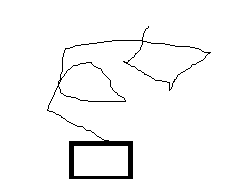
\includegraphics[scale=.7]{content/img/space_antenna}
\caption{Image of the NASA Antenna \cite{paper:ev4}}
\label{fig:nasa_antenna}
\end{figure}

\subsection{Neuro-evolution by augmenting topologies}
Neuro-evolution by augmenting topologies(NEAT) is a method for evolving 
Artificial Neural Networks(ANN) first introduced by Stanley and 
Miikkulainen\cite{stanley2002evolving}.
It evolves not only the weights of the connections in the network, but also the 
topology of the network.

NEAT employs techniques such as historical marking, speciation, and 
complexiation in order to avoid some of the shortcomings of previous methods.
By using historical markings NEAT is able to make \emph{``meaningful crossover 
between individuals with different
genetic length''}\cite[p.~50]{Floreano2008}.
Speciation allows NEAT to \emph{``protect topological innovations
that may initially display lower fitness but later
develop into powerful solutions''}\cite[p.~50]{Floreano2008}, and complexiation 
makes NEAT \emph{``produce networks of increasing complexity
starting from simple ones''}\cite[p.~50]{Floreano2008}.

The experiments carried out by Stanley and Miikkulainen show that NEAT 
outperforms previous methods by upward a factor of 
25\cite[p.~2]{stanley2002evolving}.
\subsection{Compositional Pattern Producing Networks}
\label{sec:cppn}
Compositional Pattern Producing Networks(CPPN) are a variation of regular ANNs 
introduced by 
Stanley\cite{Stanley2007}.
CPPNs use function composition in an effort to obtain repetition, symmetry, and 
regularities in the produced phenomes, see figure~\ref{fig:cppn}.
\begin{figure}[ht]
\centering
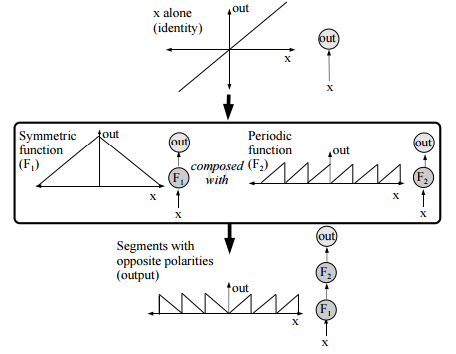
\includegraphics[width=.9\columnwidth]{cppn}
\caption{Composing two functions to obtain a single function which has multiple 
regularities \cite{Stanley2007}}
\label{fig:cppn}
\end{figure}

The evolution of CPPNs can be done using a variant of NEAT, 
CPPN-NEAT.
Specifically, where NEAT only operates with a network consisting of 
sigmoid-functions, CPPN-NEAT uses a range of different functions and chooses 
one at random when a new node is introduced into the network.
Furthermore, when determining if two individuals belong to the same species, 
the difference in which activation functions their hidden nodes use is taken 
into consideration.

CPPNs are of interest to our solution because of their symmetry producing 
properties.
%Stanley presented some experiments which used CPPNs to evolve two-dimensional 
%images.
%The input to these networks were the x- and y-coordinates of the images, and 
%the single output produced by the CPPN was used to colour the pixel at the 
%given coordinate.

\subsection{Generative Evolution of tables}
Hornby evolved tables in 2006 (see~figure~\ref{fig:hornby_tables}), using
generative encodings to to achieve reuse of similar sub-structures.
In Hornby's study, the optimisation parameters were height of the support
structure, stability of the structure, and maximization of surface area.
\begin{figure}[ht]
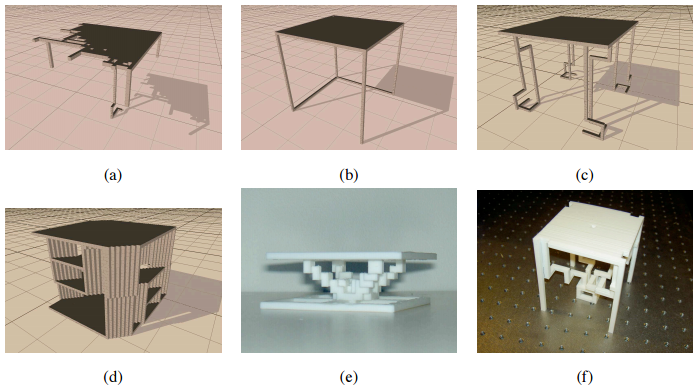
\includegraphics[scale=.6]{content/img/tables}
\caption{Image of Hornby tables\cite{paper:ev4}}
\label{fig:hornby_tables}
\end{figure}

While evolution of tables is similar to evolution of seating, they are
inherently different in the sense that maximized surface area might not be ideal
for a chair. Nor would very high legs be optimal, since the physical
attributes of humans usually constrain us to some specific height range which is
optimal for the average persons seating comfort.

\subsection{Interactive Evolutionary Computation}
Takagi describes in his survey from 2001\cite{Takagi2001}, how there are some 
\emph{``systems whose optimization indexes are difficult to 
specify''}\cite[p.~1275]{Takagi2001}.
For such systems it is beneficial to use a human subject to evaluate the outcome
of the Evolutionary Computation(EC). This method is called Interactive
Evolutionary Computation(IEC).

IEC is an ideal choice for furniture design, since the parameters of aesthetic
design are \emph{very} difficult to specify.

\subsection{Evolving 3D objects with CPPNs}
In their paper from 2011 Clune and Lipson describe how they use CPPNs to evolve 
3-dimensional objects\cite{Clune:2011:EOG:2078245.2078246}.
They describe how they encode the 3D objects with CPPNs by feeding the CPPN 
with three inputs, one each for the dimensions in a 3 dimensional Euclidean
voxel space.
The single output of the CPPN for the given coordinates is checked against a
threshold, and if it is above the threshold then the voxel in those coordinates
is considered full, otherwise it is considered
empty\cite[p.~5]{Clune:2011:EOG:2078245.2078246}. They combine this encoding
with IEC to evolve symmetrical 3D images. Examples of the figures they evolved
can be seen in figure~\ref{fig:3dobjects}.
\begin{figure}[ht]
\centering
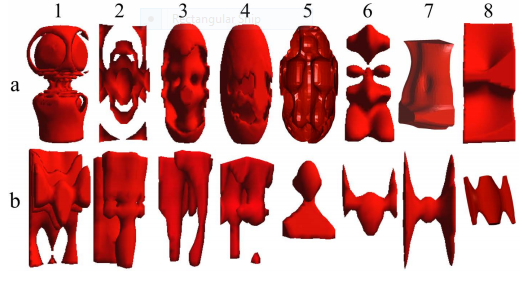
\includegraphics[width=.9\columnwidth]{3d_cppn}
\caption{Examples of the 3D images presented in 
\cite{Clune:2011:EOG:2078245.2078246}}
\label{fig:3dobjects}
\end{figure}

